\documentclass[11pt]{article}
\usepackage[margin=1in]{geometry}
\usepackage{graphicx}
\usepackage{amsmath}
\usepackage{hyperref}
\usepackage{float}

\title{CS285 Assignment 3: Q-Learning and Actor-Critic Algorithms}
\author{Xiaolei Chu (Student ID: 3038525739)}
\date{\today}

\begin{document}
\maketitle

% ============================================================
\section{Deep Q-Learning}

\subsection{Basic Q-Learning (Section 2.4)}

We trained a DQN agent on CartPole-v1. As shown in Figure~\ref{fig:cartpole}, the agent reaches the maximum return of 500 during training, confirming a correct DQN implementation.

\begin{figure}[H]
\centering
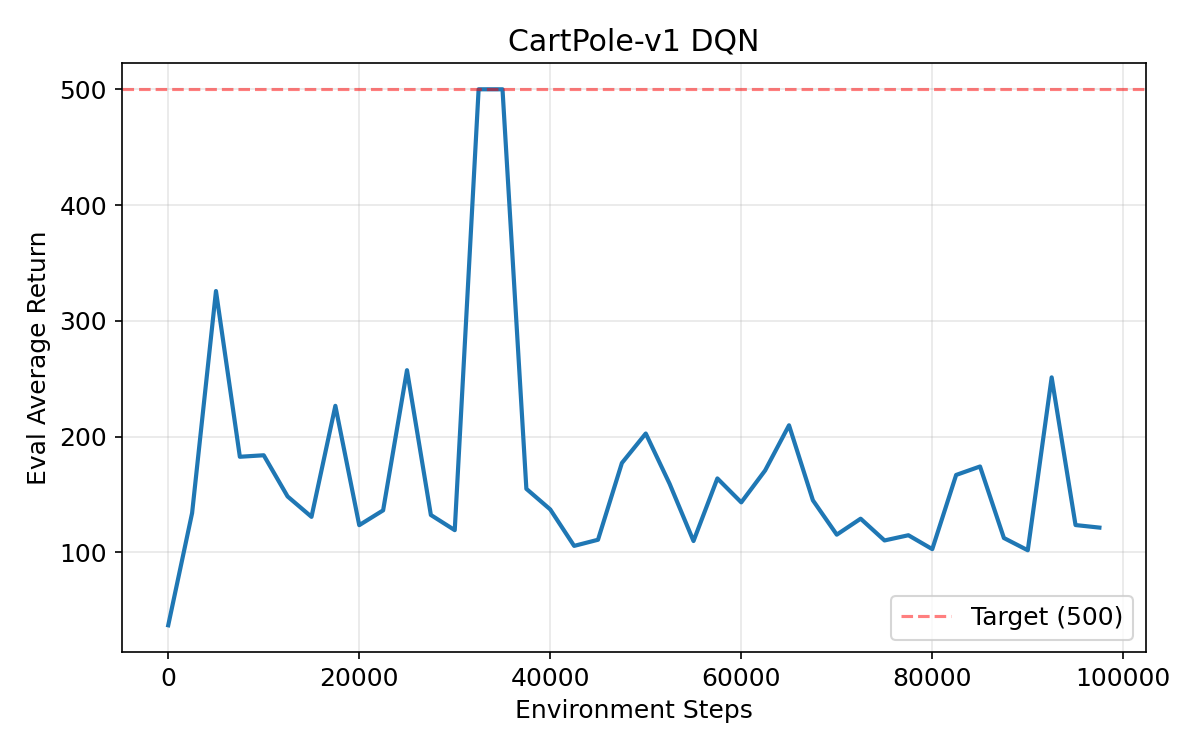
\includegraphics[width=0.75\textwidth]{report_fig1_cartpole.png}
\caption{CartPole-v1 DQN: Eval average return over environment steps. The agent reaches the maximum possible return of 500.}
\label{fig:cartpole}
\end{figure}

\subsection{Double Q-Learning (Section 2.5)}

\subsubsection{LunarLander-v2}

We trained a Double DQN agent on LunarLander-v2. As shown in Figure~\ref{fig:lunarlander}, the agent achieves a return above 200 during training (peak: 275.2), meeting the expected threshold.

\begin{figure}[H]
\centering
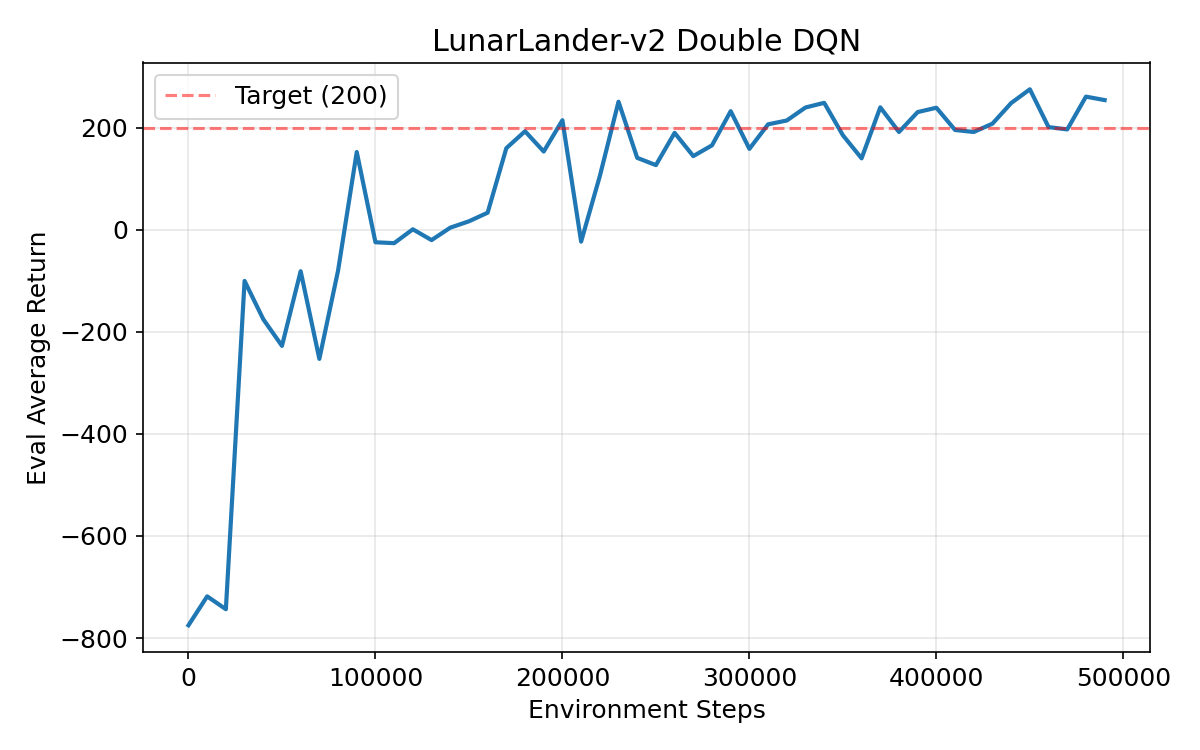
\includegraphics[width=0.75\textwidth]{report_fig2_lunarlander.png}
\caption{LunarLander-v2 Double DQN: Eval average return over environment steps.}
\label{fig:lunarlander}
\end{figure}

\subsubsection{MsPacman}

We trained DQN with double-Q learning on MsPacman. Figure~\ref{fig:mspacman} shows both the training return and eval return over training steps. The agent achieves a peak eval return of 3315, well above the 1500 target.

\begin{figure}[H]
\centering
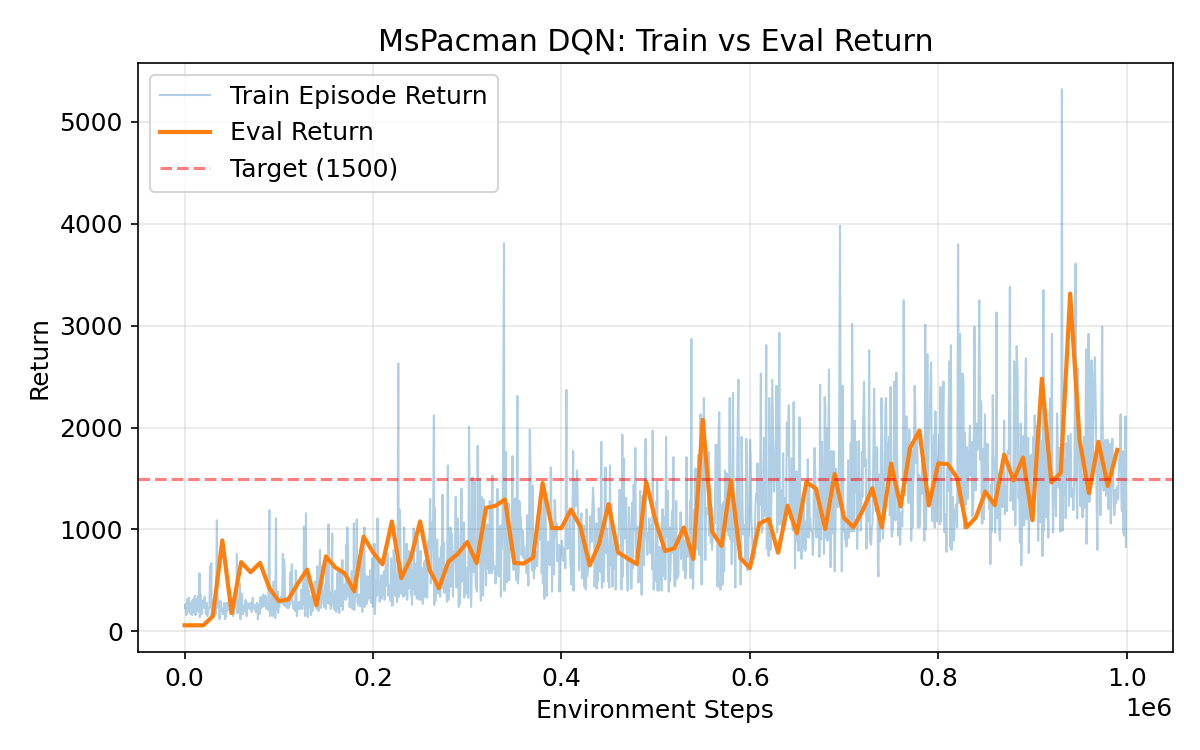
\includegraphics[width=0.75\textwidth]{report_fig3_mspacman.png}
\caption{MsPacman DQN: Raw training episode return (\texttt{Train\_EpisodeReturn}) and evaluation average return (\texttt{Eval\_AverageReturn}) plotted together.}
\label{fig:mspacman}
\end{figure}

\textbf{Explaining the difference between train and eval returns:} The two curves differ because they are measured under different policies and with different amounts of averaging. During training, \texttt{Train\_EpisodeReturn} is the return of a single online episode collected with an $\epsilon$-greedy policy, so it is much noisier and is affected by ongoing exploration. During evaluation, \texttt{Eval\_AverageReturn} is computed by running multiple evaluation episodes with the greedy policy (equivalently $\epsilon=0$ in our implementation) and averaging their returns, so it is much smoother. As a result, the curves do not need to match, and either one can be higher at different stages of training. In this run, the early training episodes are mostly around 200--330 while the eval return stays at 60 for the first 20k steps, and later the eval curve improves sharply once the learned policy becomes effective.

\subsection{Hyperparameter Experiment (Section 2.6)}

We chose to experiment with the \textbf{learning rate} on LunarLander-v2, testing four values: $1 \times 10^{-2}$, $1 \times 10^{-3}$ (default), $5 \times 10^{-4}$, and $1 \times 10^{-4}$.

\begin{figure}[H]
\centering
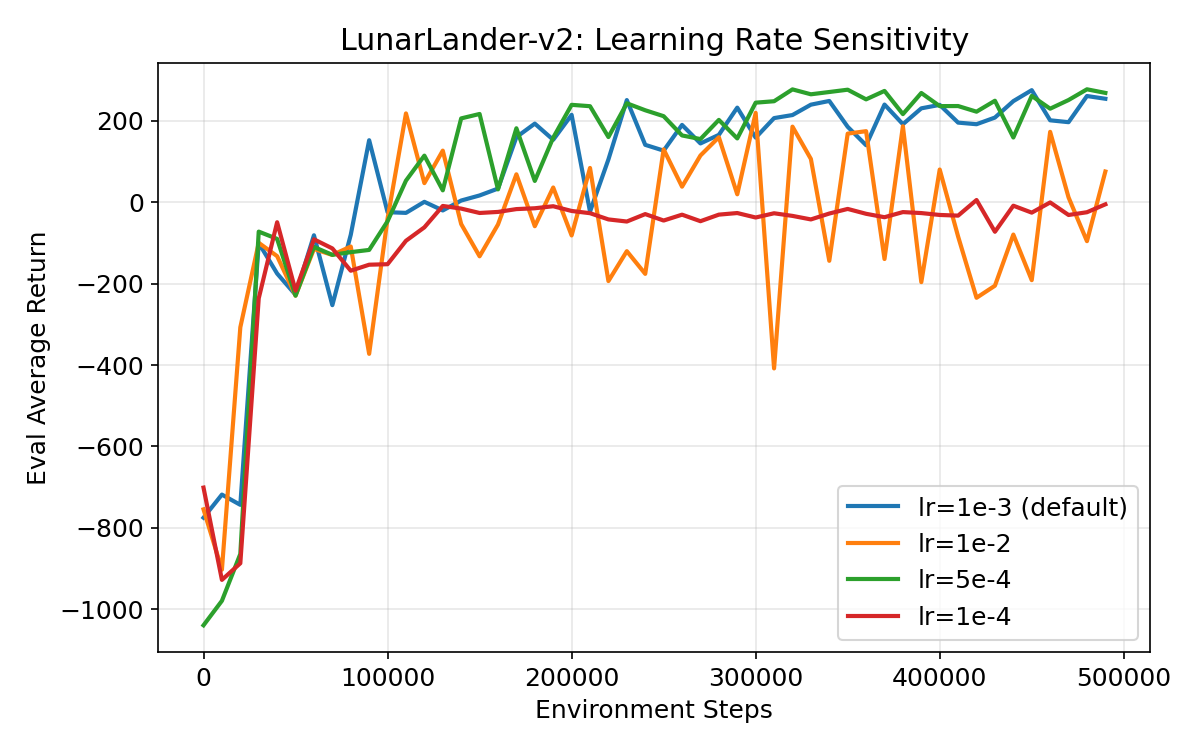
\includegraphics[width=0.75\textwidth]{report_fig4_lunarlander_lr.png}
\caption{LunarLander-v2: Learning rate sensitivity. We chose the learning rate because it directly controls the magnitude of gradient updates and is one of the most critical hyperparameters in deep RL. Too large a learning rate (lr=$1 \times 10^{-2}$) causes instability, while too small (lr=$1 \times 10^{-4}$) leads to extremely slow learning that fails to converge within the training budget. The default lr=$1 \times 10^{-3}$ and lr=$5 \times 10^{-4}$ both achieve good performance, with lr=$5 \times 10^{-4}$ performing slightly better (peak 277.4 vs 275.2).}
\label{fig:lr_sweep}
\end{figure}

% ============================================================
\section{Soft Actor-Critic (SAC)}

\subsection{Actor Update with Reparametrization (Section 3.4)}

We trained SAC on HalfCheetah-v4 with a fixed entropy coefficient (temperature parameter) of $\beta = 0.1$. As shown in Figure~\ref{fig:halfcheetah}, the agent achieves a peak eval return of 9254, well above the 6000 target.

\begin{figure}[H]
\centering
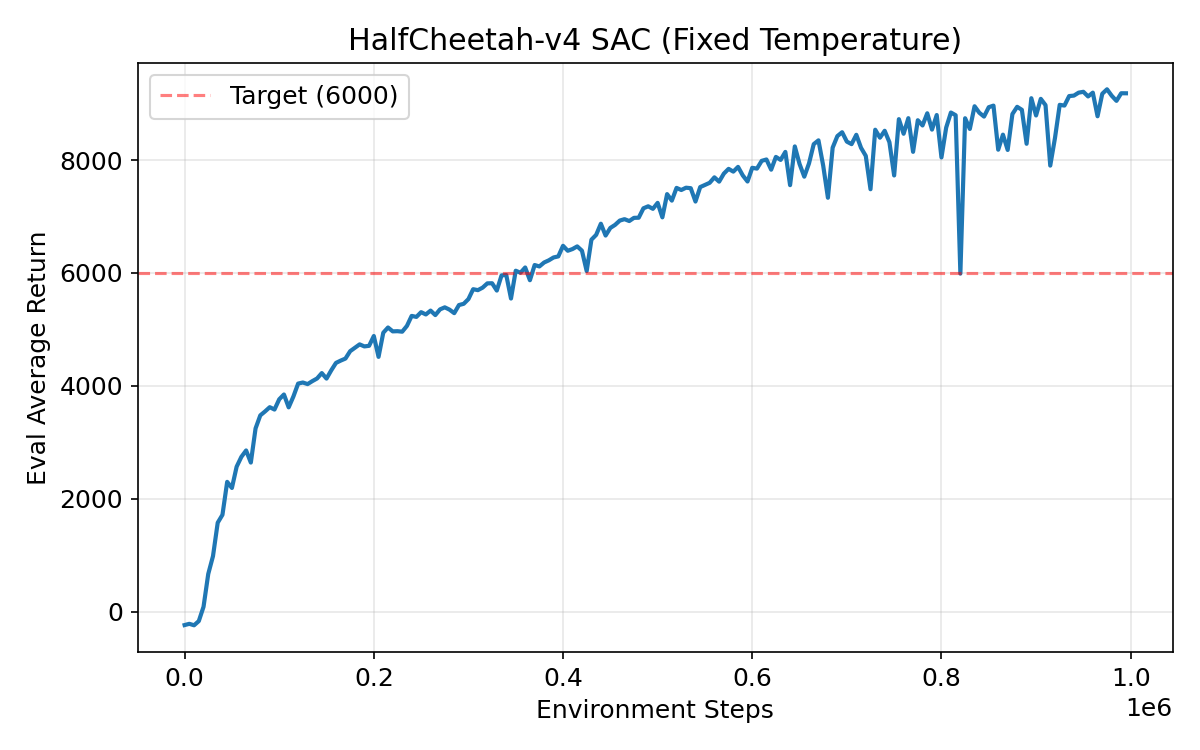
\includegraphics[width=0.75\textwidth]{report_fig5_halfcheetah_sac.png}
\caption{HalfCheetah-v4 SAC with fixed entropy coefficient $\beta = 0.1$: Eval return over environment steps.}
\label{fig:halfcheetah}
\end{figure}

\subsection{Automatic Temperature Tuning (Section 3.5)}

Figure~\ref{fig:autotune} compares fixed-coefficient and auto-tuned SAC on HalfCheetah-v4, and shows the evolution of the learned entropy coefficient $\alpha$ over training.

\begin{figure}[H]
\centering
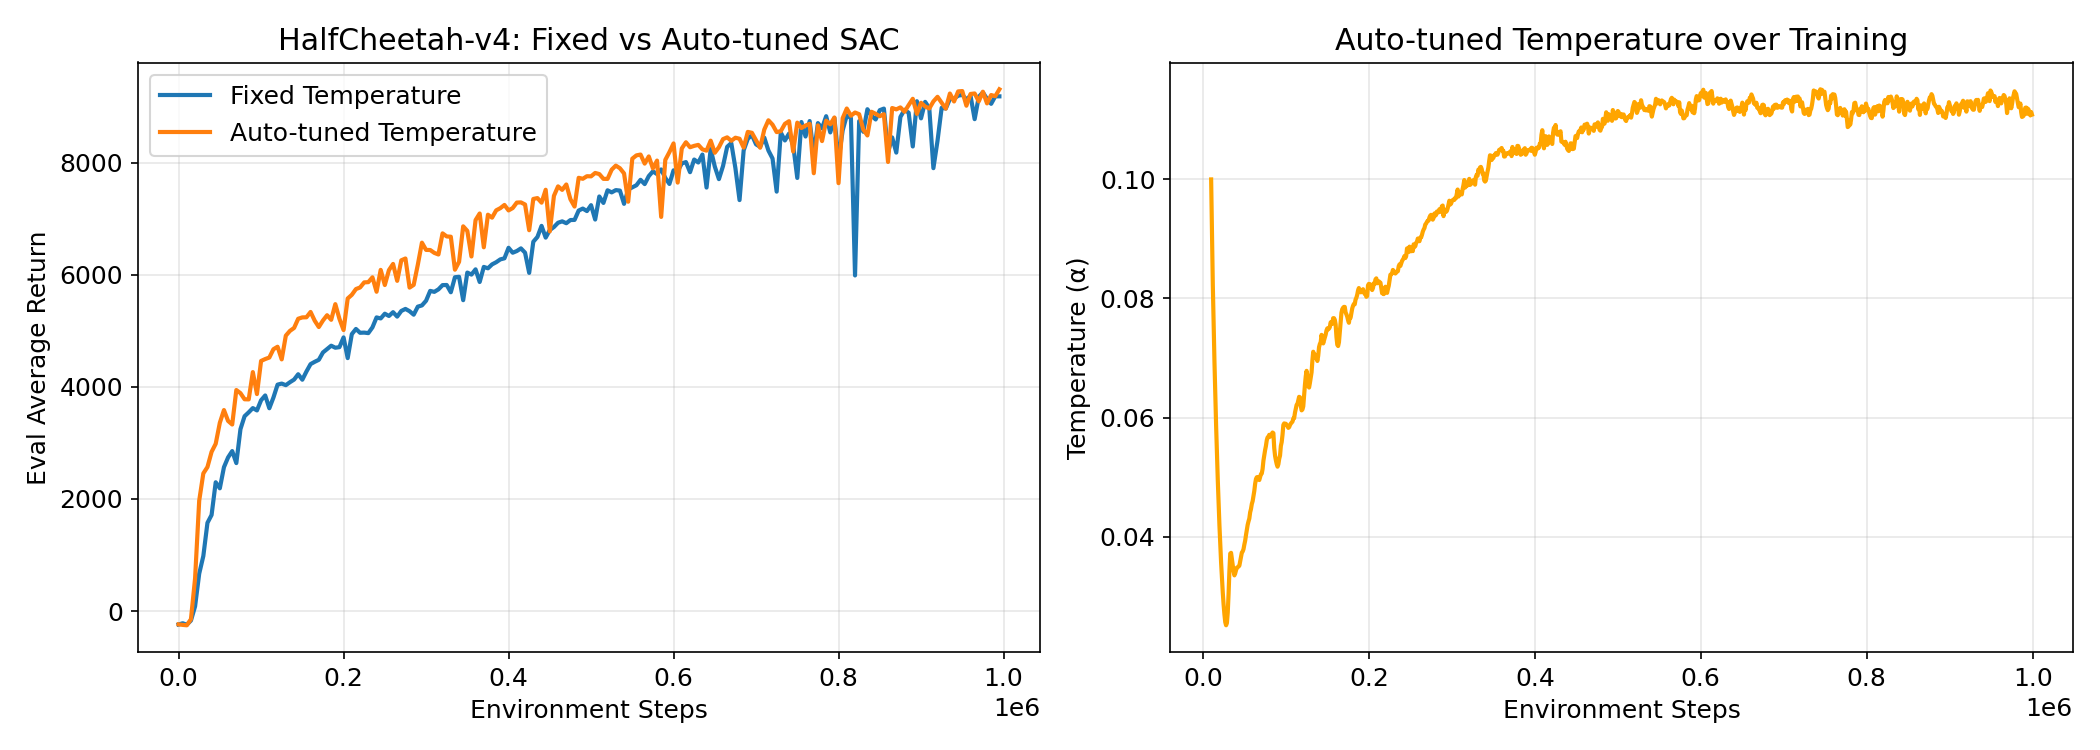
\includegraphics[width=\textwidth]{report_fig6_halfcheetah_autotune.png}
\caption{Left: Eval return comparison between fixed ($\beta=0.1$) and auto-tuned SAC on HalfCheetah-v4. Right: Learned entropy coefficient $\alpha$ over training for the auto-tuned run.}
\label{fig:autotune}
\end{figure}

\textbf{Does auto-tuning improve or achieve comparable performance to the fixed temperature?}
Auto-tuning achieves comparable performance to the fixed entropy coefficient setting. Both reach peak returns around 9250--9300, with the auto-tuned version showing slightly smoother learning in the early stages. Since the fixed coefficient ($\beta = 0.1$) is already well-tuned for HalfCheetah, the main advantage of auto-tuning is eliminating the need for manual coefficient selection.

\textbf{How does the temperature evolve during training?}
Here, ``temperature'' refers to the entropy coefficient $\alpha$ in the SAC objective. It initially drops sharply from 0.1 to approximately 0.025 in the first $\sim$100k steps, then gradually increases back to around 0.11 where it stabilizes for the remainder of training.

\textbf{Why might the temperature change in this particular way for HalfCheetah?}
The learned entropy coefficient is adapting to enforce the target entropy constraint. Early in training, the policy has very high entropy, so the dual update decreases $\alpha$ and reduces the entropy bonus. Later, as the policy becomes more concentrated and its entropy falls toward the target, $\alpha$ increases again to encourage enough stochasticity. The eventual stabilization around 0.11 indicates that the auto-tuning procedure has found a coefficient that keeps the policy entropy near the target value. For HalfCheetah's 6-dimensional action space, this target is $\mathcal{H}_{\text{target}} = -6$.

\subsection{Stabilizing Target Values (Section 3.6)}

Figure~\ref{fig:hopper} compares single-Q and clipped double-Q on Hopper-v4.

\begin{figure}[H]
\centering
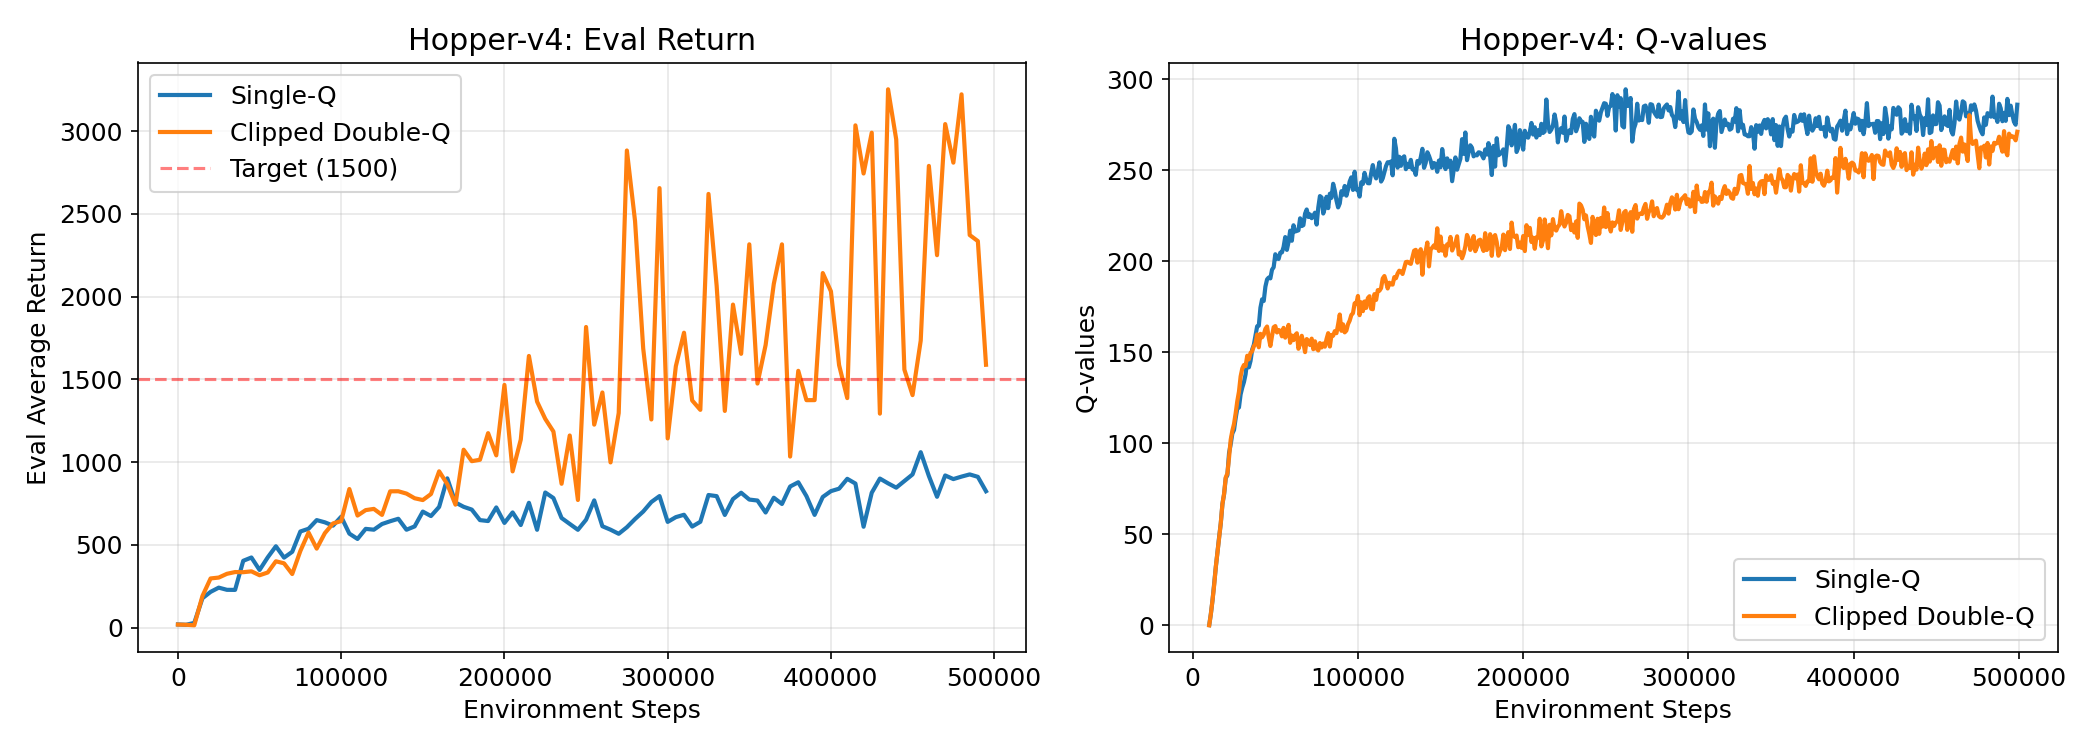
\includegraphics[width=\textwidth]{report_fig7_hopper.png}
\caption{Hopper-v4: Left: Eval return for single-Q vs clipped double-Q. Right: Q-values over training.}
\label{fig:hopper}
\end{figure}

\textbf{Which one works best?}
Clipped double-Q significantly outperforms single-Q. The clipped double-Q agent achieves a peak return of 3252, while the single-Q agent only reaches 1060.

\textbf{Discussion of overestimation bias:}
The Q-values plot clearly illustrates the overestimation problem. The single-Q agent's Q-values grow substantially larger than those of the clipped double-Q agent, despite achieving much lower actual returns. This is a classic symptom of overestimation bias: the single critic bootstraps from its own potentially overestimated values, creating a feedback loop that drives Q-values to unrealistically high levels. These inflated Q-values mislead the actor into taking suboptimal actions, resulting in poor performance.

The clipped double-Q approach mitigates this by using $\min(Q_{\phi'_A}(s', a'), Q_{\phi'_B}(s', a'))$ for the target value computation. Since two independently trained critics are unlikely to overestimate the same state-action pairs simultaneously, taking the minimum provides a more conservative and accurate value estimate. This leads to more stable training and substantially better policy performance, as evidenced by the much higher eval returns despite lower Q-value estimates.

\end{document}
